\documentclass{standalone}
\usepackage{polyglossia}
\setdefaultlanguage{vietnamese}
\setotherlanguages{english}
\usepackage{fontspec}
\usepackage{
    amsmath, 
    amsfonts, 
    amssymb
}
\usepackage{unicode-math}
% \setmainfont{STIX Two Text}
% \setmathfont{STIX Two Math}
\usepackage{xcolor}
\usepackage{tikz}
\usepackage{amsmath} % Công thức toán
\usetikzlibrary{arrows, shapes}
\begin{document}
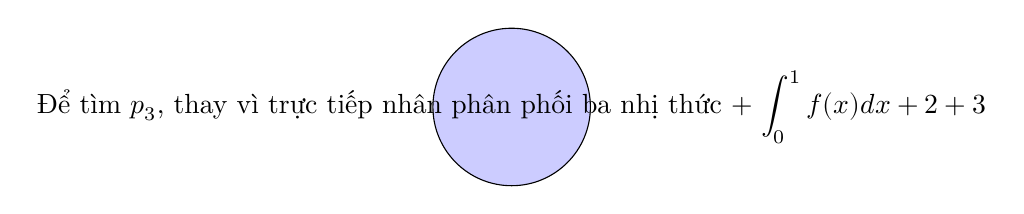
\begin{tikzpicture}
  \draw[fill=blue!20] (0,0) circle (1cm);
  \node at (0,0) {Để tìm $p_3$, thay vì trực tiếp nhân phân phối ba nhị thức + $\displaystyle\int_0^1 f(x)dx +2+3$};
\end{tikzpicture}
\end{document}